\chapter{Finding What the Detector Missed}\label{ch:recall}

\section{Introduction}\label{sec:recall-intro}
\epigraph{Far better an approximate answer to the right question, which is often vague, than an exact
answer to the wrong question, which can always be made precise.}{John Tukey, \emph{The Future of Data
Analysis} \citeyearpar[p.~13]{tukey1962}}

At the best operating point of our YOLO pipeline, about a third of the annotated filaments went
unmatched: there were 465 false negatives against 860 true positives. Recall is therefore where most
of the missing score lies. However, a filament can be missed for three quite different reasons, and
each calls for a different remedy.
\begin{itemize}[leftmargin=*,itemsep=2pt]
\item The detector never proposed anything at that location. The remedy is a better detector, or a
new source of proposals.
\item The detector proposed a good mask, and the confidence threshold discarded it. The remedy is a
\keyterm{verifier} that rescues good candidates with low confidence.
\item The detector proposed a mask on the right object, but the mask was too poor to reach an IoU of
0.5. The remedy is better boundaries (Chapter~\ref{ch:post}).
\end{itemize}

In Sections~\ref{sec:recall-orphans} and~\ref{sec:recall-stages} we measure how often each of these
cases occurs. Section~\ref{sec:recall-arith} works out how accurate a verifier must be before it can
help, and Section~\ref{sec:recall-verifiers} describes the verifiers that we built.
Sections~\ref{sec:recall-physics} and~\ref{sec:recall-semantic} try two other sources of evidence,
the physics of the image and a semantic segmentation model, and Section~\ref{sec:recall-summary}
summarises what we learned.

\section{Seen, unseen, or disbelieved?}\label{sec:recall-orphans}
Our first measurements concerned the false positives. In exp014 we called a prediction an
\keyterm{orphan} if no annotated filament overlapped it even at an IoU of 0.10. Against a given
annotator, 19.8\% of the detector's predictions were orphans. On the photographs with several
annotators, 19.4\% of one annotator's filaments were orphans with respect to a second annotator. In
other words, the detector's unacknowledged predictions occurred at the same rate as one expert's
unacknowledged filaments occur for another expert. More directly, 87 of the detector's orphans had
been drawn by a \emph{different} annotator of the same photograph.

Our notes then extended this conclusion to the misses, claiming that they too were mostly caused by
label noise. That extension was wrong, as exp016 showed by examining the whole pool of candidates,
down to a confidence of 0.05, instead of only the predictions that were emitted:
\begin{center}\small
\begin{tabular}{@{}lcc@{}}
\toprule
validation filaments (1,325) & count & share \\
\midrule
some candidate in the pool matches it at IoU 0.5 & 1,102 & 83.2\% \\
\quad of which already above the threshold of 0.35 & 797 & \\
candidates in the pool overlap it, but never reach IoU 0.5 & 195 & 14.7\% \\
no candidate in the pool touches it at all & 28 & 2.1\% \\
\bottomrule
\end{tabular}
\end{center}
Only 2.1\% of the filaments were invisible to the detector. Most of the misses had been \emph{seen
and disbelieved}: 305 filaments had a matching candidate that the threshold discarded. A result
about the false positives had been generalised to the false negatives, where it did not hold.

\section{The error, stage by stage}\label{sec:recall-stages}
We made the most careful version of this measurement later, on the two-model YOLO ensemble. In exp129
and exp132 we asked, for every annotated filament, how good the best candidate anywhere in the pool
was, with no confidence floor, no minimum area and no painting, but with the masks eroded as the
pipeline emits them (Figure~\ref{fig:recall-stages}).

\begin{figure}[t]
\centering
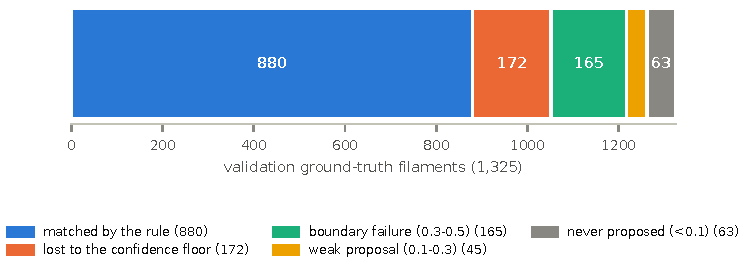
\includegraphics[width=\textwidth]{figures/fig_stages.pdf}
\caption{Every validation filament, classified by the best candidate that the pool holds for it. Most
filaments are matched by the deployed rule. The next largest groups are those whose good candidate
was discarded by the confidence floor, and those whose candidate lies on the right object but with a
boundary too poor to match. Few filaments were never proposed.
\generatedby{book/make\_book\_figures.py:fig\_stages}}
\label{fig:recall-stages}
\end{figure}

Of the filaments that the deployed rule missed, 172 had a good candidate below the confidence floor,
165 had a candidate on the right object with an IoU between 0.3 and 0.5, 45 had only a weak
candidate, and 63 (4.8\% of all filaments) were never proposed. Oracles on the uneroded pool put a
value on each remedy. Fixing the emission perfectly, that is, admitting exactly the good candidates
that the floor discarded, would raise validation PQ by $+0.050$. Fixing the boundaries of the group
with IoU between 0.3 and 0.5 would add $+0.059$, and doing both would add $+0.101$.

A companion audit, exp130, asked why the good candidates were lost. Of the 203 filaments whose best
raw candidate had an IoU above 0.5 but which nevertheless ended up unmatched, 168 (83\%) fell below
the confidence floor, 13 fell below the minimum area, 12 were destroyed by the erosion, and 10 lost
their pixels to a mask with a higher score during painting. The confidence floor was therefore the
stage that mattered.

This analysis corrected an earlier error. Before exp129, our notes had stated that 284 missed
filaments ``have zero overlap with any prediction'', and had concluded from this that the problem
was entirely one of detection. The 284 filaments had no overlap with the \emph{emitted} predictions,
which are what remains after the confidence floor has already discarded much of the evidence. In the
full pool, only 65 of them had never been proposed. Whenever we quote a number, we must know at which
stage of the pipeline it was measured.

\section{The arithmetic of admitting candidates}\label{sec:recall-arith}
Suppose that a verifier admits $k$ discarded candidates that are correct, with a mean IoU of $q$,
and $m$ that are not. Equation~\eqref{eq:metric-breakeven} of Chapter~\ref{ch:metric} says that the
score improves only if the verifier's precision exceeds $\PQ/(2q)$. Figure~\ref{fig:recall-breakeven}
plots this bar as a function of $q$.

\begin{figure}[t]
\centering
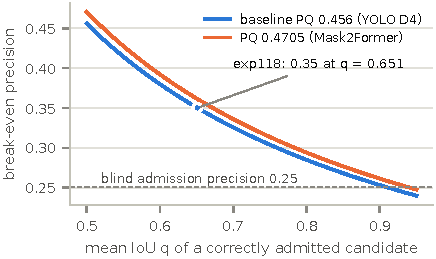
\includegraphics[width=0.62\textwidth]{figures/fig_breakeven.pdf}
\caption{The precision that a verifier needs before the candidates it admits raise PQ, as a function
of the mean IoU $q$ of the correct admissions. Admitting candidates blindly, by lowering the threshold,
reaches a precision of only about 0.25. \generatedby{book/make\_book\_figures.py:fig\_breakeven}}
\label{fig:recall-breakeven}
\end{figure}

In exp118 we measured both sides of this inequality on the pool of the YOLO ensemble, which held 601
candidates with confidences between 0.10 and the floor of 0.35. Lowering the floor blindly always
lowered the score:
\begin{center}\small
\begin{tabular}{@{}cccccc@{}}
\toprule
floor & PQ & added TP & added FP & precision of the additions \\
\midrule
0.35 (deployed) & 0.4559 & -- & -- & -- \\
0.30 & 0.4501 & 32 & 95 & 0.25 \\
0.25 & 0.4421 & 63 & 205 & 0.24 \\
0.20 & 0.4260 & 89 & 365 & 0.20 \\
0.10 & 0.3969 & 109 & 634 & 0.15 \\
\bottomrule
\end{tabular}
\end{center}
An oracle that admitted exactly the right candidates reached 0.4767, a gain of $+0.0208$, by admitting
132 candidates that recovered 120 misses with a mean IoU of 0.651. At this value of $q$,
Equation~\eqref{eq:metric-breakeven} sets the bar at a precision of 35\%, but a precision of 35\%
only breaks even. To reach 0.472, the verifier needed a precision of about 50\% at around 120
admissions, whereas blind admission achieved 24 to 25\%. A useful verifier therefore had to roughly
double the precision of the candidates that it chose.

\section{Verifiers}\label{sec:recall-verifiers}
A \keyterm{verifier} is a second model that re-scores the detector's candidates, using evidence that
the detector's confidence does not already contain. We built several.

\subsection{Hand-made features}\label{sec:recall-features}
Our first verifier was a gradient-boosted classifier~\citep{friedman2001} over four shape features: area, elongation,
distance from the limb, and solidity. We trained it with the photographs grouped, so that no
photograph appeared in both the training and the validation folds. It lost to the raw confidence by
0.017. A re-ranker built on fourteen cuts through each mask's field of logits ranked the candidates
slightly better than the confidence did (an average precision of 0.7248 against 0.7150), yet even its
most conservative promotion added 23 false positives and no true ones.

Later screens on the ensemble's pool found no single feature that could verify a discarded
candidate. The best was the detector's own score, with an AUC of 0.64, followed by the distance from
the limb, with an AUC of 0.60; candidates near the centre of the disk were more often real. A logistic
regression~\citep{murphy} over nine features, fitted out of fold, recovered 8\% of the admission ceiling
($+0.0017$). Gradient boosting on the same features memorised the 132 positive examples and lost.
Whether a second architecture also proposed the candidate was the best single feature we found, with
an AUC of 0.688, and it still did not yield an operating point with a positive gain.

\subsection{The crop verifier and the wrong question}\label{sec:recall-crop}
In exp025 to exp027 we trained a small convolutional network, with 827,000 parameters, on 13,413 crops
of $128\times128$ pixels. Each crop had two channels: the photograph and the proposed mask. For
candidates with confidence below 0.30, its average precision was 0.576, against 0.455 for the
detector's confidence and a base rate of 0.344. Of its top 100 candidates in this range, 72\% were
real filaments. Yet when we used it as an emission rule, it added 100 true positives at the cost of
496 false positives, a precision of 17\%.

The gap between 72\% and 17\% was caused by a decision about labels. We had labelled a crop as
positive if \emph{any} annotator of the photograph had drawn a filament there, reasoning that
labelling against a single annotator would teach the model to call another annotator's filament a
mistake. But PQ scores each annotation record separately, against \emph{one} annotator
(Figure~\ref{fig:recall-labels}). The verifier had learned to answer the question ``would somebody
draw this?'', whereas the metric asks ``did this person draw it?''.

\begin{figure}[t]
\centering
\begin{tikzpicture}[
  panel/.style={draw=inkmuted, line width=0.6pt, fill=gridline!40, minimum width=3.2cm,
                minimum height=1.9cm, rounded corners=2pt},
  truth/.style={line width=6pt, line cap=round, draw=inkmuted!55},
  cand/.style={line width=1.2pt, draw=vizorange, dash pattern=on 3pt off 1.5pt},
  tag/.style={font=\sffamily\scriptsize\bfseries, text=white, fill=#1, rounded corners=1.5pt,
              inner sep=2.5pt}]
  \foreach \px/\ttl in {0/{record of annotator A}, 3.9/{record of annotator B}}{
    \node[panel] at (\px,0) {};
    \node[title] at (\px,1.2) {\ttl};
  }
  % annotator A drew both filaments; annotator B drew only the upper one
  \draw[truth] (-1.2,0.45) .. controls (-0.5,0.7) and (0.4,0.3) .. (1.2,0.5);
  \draw[truth] (-1.0,-0.45) .. controls (-0.4,-0.25) and (0.3,-0.55) .. (1.0,-0.35);
  \begin{scope}[xshift=3.9cm]
    \draw[truth] (-1.2,0.45) .. controls (-0.5,0.7) and (0.4,0.3) .. (1.2,0.5);
  \end{scope}
  % the same candidate on the lower filament in both records
  \foreach \px in {0,3.9}{
    \begin{scope}[xshift=\px cm]
      \draw[cand] (-1.05,-0.5) .. controls (-0.4,-0.3) and (0.3,-0.6) .. (1.05,-0.4) -- (1.05,-0.28) .. controls (0.3,-0.48) and (-0.4,-0.18) .. (-1.05,-0.38) -- cycle;
    \end{scope}
  }
  \node[tag=vizblue] at (0,-1.25) {per record: positive};
  \node[tag=vizorange!85!black] at (3.9,-1.25) {per record: negative};
  \node[box=inkmuted, text width=2.9cm, font=\sffamily\scriptsize] at (8.0,0.25)
       {``any annotator'' label: \textbf{positive} for both records};
  \node[note, text width=3.2cm] at (8.0,-0.85) {PQ scores each record on its own, so one admission is a TP in A and an FP in B};
\end{tikzpicture}
\caption{Why a verifier must be labelled per record. The dashed candidate lies on a filament that
annotator A drew and annotator B did not. Labelled ``positive if any annotator drew it'', the
candidate teaches the verifier a question that PQ never asks.
\drawnin{book/chapters/ch10\_recall.tex}}
\label{fig:recall-labels}
\end{figure}

The lesson is general. Before choosing the labels for a model, we should write down the exact
question that the metric asks of each prediction, and check that the training objective asks the same
question. Here the metric asks, for each annotation record, whether this candidate matches this
annotator's filament with an IoU above one half.

We also used the mistake as a probe of the leaderboard. If the test labels were a consensus of several
annotators, or otherwise more inclusive than those of a single annotator, then the crop verifier's
high-recall rule would transfer to the leaderboard better than its validation score suggested. We
submitted it as exp028: it emitted 1,624 instances and scored 0.041 \emph{worse} on validation. It
appeared on the leaderboard as 0.32, which is what the usual offset between validation and the
leaderboard predicts, so the test labels behave like the validation labels
(Section~\ref{sec:val-rejected}).

\subsection{The crop verifier with the right labels}\label{sec:recall-crop-fixed}
In exp134 we repeated the idea with the labels corrected. There was one example for each combination
of photograph, record and proposal, and it was positive only if the proposal matched a filament in
that record. We trained the network on 5,281 crops harvested from the training photographs, of which
19\% were positive. The inputs were well formed, and the ceiling was real: 168 of the 172 filaments
lost to the confidence floor had a proposal with an IoU above 0.5 among the crops. The model did not
learn. Its average precision on validation wandered between 0.19 and 0.25 for twenty epochs, against a
base rate of 0.18, and its loss stayed at the value that a random classifier achieves. Every admission
rule based on it lost. Two simple physical features, the contrast in darkness between the inside and
the outside of the mask, and the mask's area, were also at chance, with AUCs of 0.53 and 0.50.

Our interpretation is that, for these candidates, the detector's low confidence reflects a real
uncertainty: within a crop of 128 pixels, a real filament under a low-confidence proposal does not
look different from a false one. This statement is about the formulations we tested, namely crops of
this size and features of this kind, and we do not claim more than that.

\section{Physics and classical vision}\label{sec:recall-physics}
If the network misses filaments, perhaps physics can find them. A filament absorbs light in the \Ha{}
line, so it appears darker than the quiet disk. In exp103 we built a classical proposal stage based on
this fact, summarised in Algorithm~\ref{alg:recall-classical}.

\begin{algorithmblock}{A physics-based proposal stage (exp103)\label{alg:recall-classical}}
\item \textbf{flatten the limb darkening:} divide each pixel by the median intensity of all disk pixels at the same distance from the centre of the disk;
\item \textbf{measure local contrast:} estimate the background by heavy blurring at two scales, and keep the larger of the two differences between background and pixel;
\item \textbf{grow by hysteresis:} mark seeds where the contrast exceeds a strict threshold, and let them grow through connected pixels above a permissive threshold;
\item \textbf{keep elongated components:} keep components whose minimum-area rectangle is long compared with its width
\end{algorithmblock}

The first step removes the darkening of the disk towards the limb, which is caused by the line of
sight grazing the solar atmosphere there. If $\mathbf{c}$ is the centre of the disk, the flattened
image is
\begin{equation}
I_{\text{flat}}(\mathbf{u}) = \frac{I(\mathbf{u})}{\operatorname{median}\{I(\mathbf{u}') :
\lVert\mathbf{u}'-\mathbf{c}\rVert = \lVert\mathbf{u}-\mathbf{c}\rVert\}},
\end{equation}
after which a filament should be dark everywhere on the disk. The second step reflects the fact that a
filament is darker than its surroundings, whatever its absolute intensity. The third step, the
hysteresis thresholding of the edge detector of \citet{canny1986}, lets the faint tails of a
filament grow from its confident core, while isolated faint pixels, which touch no
seed, are discarded. The fourth step uses the fact that filaments are long and thin.
Listing~\ref{lst:recall-classical} shows the second and third steps.

\begin{lstlisting}[caption={Local contrast and hysteresis. Condensed from
\file{experiments/exp\_103\_classical/src/proposals.py}.},label=lst:recall-classical]
def local_contrast(flat, scales=(31, 101)):
    valid = (flat > 0).astype(np.float32)
    best = np.zeros(flat.shape, np.float32)
    for scale in scales:                  # background by heavy blurring, normalised by coverage
        background = (cv2.GaussianBlur(flat, (0, 0), scale / 3.0)
                      / np.maximum(cv2.GaussianBlur(valid, (0, 0), scale / 3.0), 1e-3))
        best = np.maximum(best, background - flat)      # darker than surroundings = positive
    return best * (flat > 0)

def hysteresis(contrast, high, low, disk):
    strong = ((contrast >= high) & (disk > 0)).astype(np.uint8)
    weak = ((contrast >= low) & (disk > 0)).astype(np.uint8)
    count, labels = cv2.connectedComponents(weak, connectivity=8)
    keep = np.zeros(count, bool)
    keep[np.unique(labels[strong > 0])] = True           # weak regions that touch a seed
    keep[0] = False
    return keep[labels].astype(np.uint8)
\end{lstlisting}

On three validation photographs, this stage produced one to three proposals per photograph and
covered no annotated filament at all. The thresholds were not to blame. At a seed threshold that kept
76\% of the filament pixels, the mask also kept about a third of the disk, so hysteresis grew a single
enormous blob, which the elongation filter then discarded. The contrast inside filaments overlapped
the contrast of the surrounding \keyterm{chromospheric network}, the mottled pattern of dark and bright
cells that covers the whole disk (Section~\ref{sec:data-sun}).

To quantify this, we asked the following question of several candidate quantities: if a threshold
keeps 80\% of the filament pixels, what fraction of the disk does it keep?
Figure~\ref{fig:recall-classical} shows the answers. The best quantity, a measure of ridges based on
the Hessian~\citep{lindeberg1998,frangi1998}, still kept 26\% of the disk, whereas a useful proposal stage would need to keep less than
5\%. The Hessian is the matrix of second derivatives of the image $I_\sigma$ smoothed by a Gaussian of
width $\sigma$,
\begin{equation}
\mathbf{H}_\sigma(\mathbf{u}) = \sigma^2
\begin{pmatrix} \partial_{xx} I_\sigma & \partial_{xy} I_\sigma \\ \partial_{xy} I_\sigma & \partial_{yy} I_\sigma \end{pmatrix}.
\end{equation}
On a dark line, its larger eigenvalue is large and positive, reflecting the strong curvature of the
intensity across the line, and its smaller eigenvalue is near zero, reflecting the absence of
curvature along it. The Hessian responds most strongly to lines whose width is comparable to $\sigma$,
and our test used $\sigma = 2$, 4 and 8 pixels.

\begin{figure}[t]
\centering
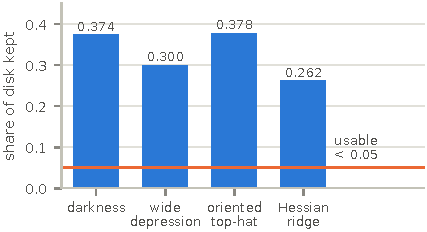
\includegraphics[width=0.62\textwidth]{figures/fig_classical.pdf}
\caption{The fraction of the solar disk that each classical quantity keeps when its threshold keeps
80\% of the filament pixels, averaged over three photographs. A usable proposal stage needs a value
well below 0.05. \generatedby{book/make\_book\_figures.py:fig\_classical}}
\label{fig:recall-classical}
\end{figure}

These tests apply each quantity \emph{globally}, over the whole disk. They do not test local evidence
of a ridge sampled in a narrow corridor ahead of the end of a detected filament, at the filament's own
width. That local use remains untested, and the global results should not be quoted against it. A
related test, exp076, used darkness, the coverage of dark pixels and elongation to rescue the
detector's weak proposals, rather than to propose new ones. Its best rule raised the number of true
positives from 860 to 882, but also raised the false positives from 397 to 446, and it lost (0.4546
against 0.4559).

\section{Semantic evidence}\label{sec:recall-semantic}
The dense models of Chapter~\ref{ch:paradigms} had lost as instance segmenters, but a semantic
probability map is independent evidence about where filaments are. We tried to use it in both
directions, to add masks and to remove them.

\paragraph{Adding masks.} In exp081 we used the frozen U-Net of exp004 to support weak proposals. A
proposal with a confidence between 0.26 and the floor was admitted when the semantic model's mean
probability inside it was at least 0.80. The validation score rose from 0.4559 to 0.4594, with true
positives rising from 860 to 891 and false positives from 397 to 438. Submitted as exp082, with 77
extra masks, it appeared on the leaderboard as 0.38, below the 0.39 of the same pipeline without them.
Two earlier probes that added masks with low confidence or small area (exp064 and exp065) had also
appeared as 0.38. The leaderboard consistently penalised additions that validation favoured by a few
thousandths.

\paragraph{Removing masks.} In exp085 we trained a new semantic model, based on a recent paper on
solar filaments by \citet{hu2026morden}. It used $5\times5$ convolutions, instance
normalisation~\citep{ulyanov2016}, parallel branches at several scales, channel gates in the manner
of squeeze-and-excitation~\citep{hu2018senet}, pooled context at several scales as in
PSPNet~\citep{zhao2017pspnet}, three input channels (the
raw image, a CLAHE version and a map of local dark contrast), a second output for the spine, and a
loss combining the focal loss~\citep{focal} with the Dice loss~\citep{vnet}. It trained in 25 minutes and reached a
Dice coefficient of 0.70 on masks and 0.64 on spines; on its own it scored a PQ of 0.3227. As evidence
for \emph{pruning}, however, it helped. In exp090 we removed a YOLO mask when the 75th percentile of
the semantic model's probability inside it was low, with a stricter bar near the centre of the disk
(0.30 within 0.65 of the radius) than near the limb (0.12). The validation score rose to 0.4606, and
the removals were correct 68\% of the time. In 500 bootstrap resamples the pruned rule beat the
baseline 93 to 95\% of the time, and on the leaderboard it appeared as 0.39, equal to our best score
at that time.

\section{What the recall work established}\label{sec:recall-summary}
The pool of candidates held most of the missing filaments, and an oracle showed that re-admitting the
right ones was worth about two hundredths. None of the verifiers that we built could pick them out
with the precision that the metric demands. Hand-made features, a crop classifier with the correct
labels, the opinion of a second architecture, physical contrast and a semantic model all fell short,
most of them far short. These measurements do not show that the task is impossible. They show that
the evidence available to these verifiers, in crops and features of the kinds we used, does not
separate a faint real filament from the surrounding network well enough. Our next step was therefore
to look for a detector whose candidates would need less rescuing.

\section*{Exercises}
\begin{exercise}{The emission rule}
Show that admitting one candidate that matches with probability $p$, with an expected IoU of $q$ when
it matches, raises PQ in expectation if and only if $pq > \tfrac12\PQ$. Relate this condition to
Equation~\eqref{eq:metric-breakeven}.
\end{exercise}

\begin{exercise}{The precision needed}
Using the table of blind floors in Section~\ref{sec:recall-arith}, compute the mean IoU $q$ of the 32
true positives added at a floor of 0.30, assuming that the numerator of PQ rose by exactly their IoUs.
Then check whether their precision of 0.25 should have raised or lowered PQ.
\end{exercise}

\begin{exercise}{Labels per record}
Write the labelling function for the verifier of exp134: given a photograph's records and one
proposal, return one label per record. How many training examples does a photograph with three
records and twenty proposals produce, and how should they be weighted so that heavily annotated
photographs do not dominate?
\end{exercise}

\begin{exercise}{A Hessian on a synthetic ridge}
Draw a dark Gaussian ridge of width $w$ on a bright background, and compute the eigenvalues of
$\mathbf{H}_\sigma$ at its centre for several values of $\sigma$. Show that the response peaks near
$\sigma \approx w$, and explain why a network of dark cells 5 to 15 pixels across also responds.
\end{exercise}

\begin{exercise}{Adding versus removing}
The rule of exp082 added 77 masks and appeared lower on the leaderboard, whereas the rule of exp090
removed masks and appeared equal. Suppose that the 90 photographs of the public leaderboard are an
independent sample, like the validation photographs. Estimate the standard deviation of the change in
the public score caused by 77 additions with a precision of 0.4, and decide whether the observed drop
is surprising.
\end{exercise}
